% !TEX root = _main.tex

\section{はじめに}

近年，音楽や映画といった時系列メディアを対象とした多様な作品分析手法が提案されている．これらの分析において，対象作品の視聴や分析方法の検討など，さまざまな要素が含まれるが，場面分けは多くの分析手法に共通する基盤的な作業である．分析者は場面分けを直感的に行う場合が多く，その基準は明確化されていないことが多い．

特に映像作品においては，鑑賞者や分析者それぞれが異なる視点を持つため，設定される場面が大きく異なることが指摘される．このような状況を踏まえ，本研究では映像作品の場面分けに着目し，場面を細分化する際に考慮される要素を分析・考察し，根拠をもって場面分けする方法を検討する．

\section{研究背景}
時系列メディアを扱った分析はさまざまな手法で行われている．分析をする上で様々な作業があるが，対象作品の場面分けは多くの分析手法に共通するものである．場面分けの手法として，自動で分割する方法やシステム分割する方法や手動で分割する方法が存在する．

自動分割の例として，PySceneDetect\cite{PySceneDetect}が挙げられる．このツールは，動画からシーンの変更点を検出して，それに基づいて動画をシーン単位で分割することができるPythonライブラリである．動画編集や分析，コンテンツ管理などに応用されている．

シーン間の変化の閾値を設定することで，視覚的に大きな変化を特定可能となり，場面分けを行う．

実際PySceneDetect使用してみると，映像の色が大きく変わった時に場面分けが行われるので，場面分けがとても細かくなる．多様な分析がある中でそのような場面分けは，そのまま扱うのではなく，グルーピングを行う場合がほとんどである．グルーピングをする一つの指標として挙げられるのは分析者が対象作品による視点である．人が対象作品を観る際，各それぞれの登場人物や起こった事象やBGMなどといった様々な視点をもって鑑賞する．メディア作品を対象として分析をする際，多様な視点を構造化していく．

本研究では，手動で分析する際，どのような基準をもって場面分けを行っているか調査を行う．調査方法として，CiNii\cite{CiNii}を利用し，手動によるメディア分析を対象とした論文を抽出・調査した．分析対象は以下の8つのカテゴリに絞った：演劇，小説，プレゼンテーション，映画，将棋，映像，作品分析，感情分析．これらの論文から，さらに「分析」と「場面分け」に関する記載があるものを抽出し，対象を絞り込んだ．

次に，抽出された論文に記載された場面分けに着目し，各分析者がどのような観点や理論に基づいて作品の場面分けを行っているのかを調査を行った．その結果，該当する論文は合計84件が抽出された．そのうち，「分析」と「場面分け」に関する記載が明確に認められる論文は12件に絞られた．これら12件の対象となるメディアのカテゴリは，映画，アニメ，ゲームシナリオ，ミステリー小説，ミュージカル，神話の6つであった．

以下で取り扱ったメディア分析を行っている論文のいくつかを例に挙げて概要，分析方法，場面分けのやり方を述べていく．


\subsection{論文例}
\subsubsection{長編アニメーション映画『崖の上のポニョ』の構造分析―2編の小さな異郷訪問譚の接合―}
\paragraph*{(1)概要}
スタジオジブリ製作における宮崎駿が関わった長編アニメーション映画には根強い人気がある．その中でも『崖の上のポニョ』を対象として構造分析を行う\cite{ponyo}．物語形式の中でも，「異郷訪問譚」の裏返し構造を用いた分析を行うことで，作品の特性を明らかにする．異郷訪問譚とは日本の代表的な異郷訪問譚である「イザナギの黄泉国訪問譚」や「浦島子」などにもみとめ られるように，古くから使用されてきた物語類型 の一つとも言え，いわゆる成長物語との関連がし ばしば指摘されてきた形式である．
\paragraph*{(2)分析方法}
物語の前半のテーマが後半では逆の順序で出現し，後半では前半の否定ないし対立という形をとる構造を裏返し構造という．その構造を援用する手法により『崖の上のポニョ』を分析していく．
\paragraph*{(3)場面分けの方法}
物語を前半と後半で分けその反対の形をとる場面の名称付けをして当てはめていく．

\subsubsection{物語の訴求分析の理論と手法及び応用事例}
\paragraph*{(1)概要}
物語は，古くから社会や文化の価値観形成に影響を与えてきた重要な要素．神話や昔話だけでなく，現代の娯楽作品（小説，コミック，アニメ，映画など）や広告，ニュース記事にも「物語」が含まれている．これらの物語は時代や文化に応じて変化し，私たちの価値観や意思決定に影響を与える\cite{sokyu}．「物語の訴求力」つまり，物語が持つ魅力や影響力を分析するための理論と手法を構築し，その意義を探ることを目的としている．
\paragraph*{(2)分析方法}
コミックの「進撃の巨人」を対象としてシーケンス分析を行っていく．シーケンス分析とは，物語が持つ「イベントの連鎖」に注目し，その構造を明らかにする分析手法である．この手法は，特に神話や民話などに見られる繰り返しのパターン（スキーマ）を抽出し，それがどのように物語全体の訴求力を形成しているかを検討することを目的とする．シーケンス分析は，物語の中に隠されたテーマや価値観を発見し，それを科学的に解明するための有力な手段となる．
\paragraph*{(3)場面分けの方法}
信頼や疑念といったスキーマを設定し，その内容に当てはまる場面を簡潔な言葉で設定した．

\subsection{結果}
場面設定に関しては，明確な理由に基づいて設定されているものと，そうでないものが存在することが分かった．明確な理由をもって場面が設定されている場合，その分析方法は，特定の条件を設け，その条件に従って場面を分類していくという形態が多かった．また，推理小説などの特定のジャンルにおける分析では，事件や推理の進行など，明確なパートが存在するため，それらのパートに場面を当てはめる傾向が見られた．

一方，物語の中で場面転換や登場人物の増減などの物理的な変化に基づいて場面が分割されることはあったが，それ以上に細かい場面設定が行われることは少なかった．このように，場面の分け方にはジャンルや分析方法によって異なる特徴が見られることが確認された．

\subsection{考察}
論文調査を通じて，分析対象となる作品全体を明確な理由をもって場面分けしている分析事例は確認されなかった．この結果から，分析者は場面分けそのものを必ずしも重要視しているわけではない可能性が示唆される．

場面分けは，あくまで分析対象作品のどの部分を指しているかを可視化するための手段として機能しているに過ぎず，その行為自体に特別な意味を持たせる必要性を感じていないと考えられる．そのため，場面分けのプロセスは多くの場合において直感的に行われているのではないかと推察される．

以上の考察を踏まえると，場面分けの方法や基準を体系化する必要性は分析の目的次第で異なり，必ずしも全ての分析において不可欠な要素ではない可能性があると考えられる．

\section{分析の入出力}
分析の流れとして，入力があり，処理をして出力するというものである．メディア作品を対象とする場面分けの入出力は，入力は映像になり，視点によって行う処理が変わり，場面分けが出力される．

以下で調査によって選定された論文の視点と出力をまとめていく．
\begin{itemize}
\item
物語自動生成のための推理小説中の伏線分類\cite{suiri}

視点：事件や推理に関しての伏線

出力：シーンの機能とシーンに含まれる伏線の抽出・伏線として示唆される方法と伏線によって示唆される情報に分けて抽出
\item
物語の訴求構造分析の理論と手法及び応用事例

視点：シーケンス（イベントの連鎖）の繰り返し

出力：物語の登場人物が「何に困り」「何を回復しようとし」「何を獲得しようとし」最後に「何を獲得/回復するか」を抽出
\item
長編アニメーション映画『崖の上のポニョ』の構造分析

視点：物語の前半と後半との裏返しの関係

出力：物語の後半要素が前半要素の裏返しとなり，物語の後半要素の出現順序は，それぞれ対応する前半要素の逆の順序を抽出
\item
神話物語と神話を原型にした現代物語の構造比較\cite{sinwa}

視点：物語の課題解決

出力：物語の課題のカテゴリ分けし定義づけをおこない，その出現頻度を出力
\item
ロールプレイングゲームシナリオにおける クエスト構造に着目した物語分析\cite{rpg}

視点：イベント（クエスト）の繰り返し

出力：ゲームシナリオの頻出パターンの抽出
\item
ネットワーク分析を用いたミステリー小説における場面の依存関係の分析\cite{misuteri}

視点：場面間の依存関係

出力：場面情報（項目・説明）の抽出
\item
オンライン小説におけるキーワードの時系列傾向分析\cite{onrain}

視点：キーワード

出力：キーワードの出現頻度を時系列順に出力
\item
アニメ視聴による心理学的体験の構造化\cite{anime}

視点：心理学的体験

出力：視聴により生じたアニメの心理学的体験を出力
\end{itemize}
\subsection{視点・出力共通点}
視点では，場面同士の関係を視点としているものが多くみられた．

出力では，各それぞれの分析で設定した要素の頻度を出力していたものが共通点として挙げられる．


\section{同一作品の解釈}
これまでで，さまざまな作品を対象とした分析を調査したが，同一作品を複数の視点で分析するものは存在しなかった．そこで同一作品を複数の視点で場面分けした場合どのような解釈になるのか疑問に思った．

そこで同一作品を複数人が場面分けすることで，複数の視点で解釈する方法が可能となるのではないかと考えた．本研究では，
場面分けの比較実験を行い分析することで，
―――――――――――

\subsection{対象作品}
1940年から1958年までに公開された短編アニメーションシリーズのトムとジェリー\cite{tom}から4作品を対象とする．トムとジェリーを対象とした理由としては，登場人物が少なく，一話完結で，短編かつ話が数多く存在したためである．対象とする話としては，The Two Mouseketeers・The Cat Concerto・The Missing Mouse・Mouse Troubleの4作品である．

\subsection{分析方法}
分析方法として，被験者を用意してそれぞれ同じ映像作品を複数話鑑賞してもらい場面分けを行っていく．本研究における被験者は、18歳から20歳までの男女計3名となる．場面分けの記入はGoogleのスプレットシートを利用する．場面分けに対していくつか条件を与えた．一つ目は場面に名称についてである．分析する際分析者が見てどの場面か把握出来ないと分析自体破綻するため最低限主語と動詞をいれてもらい誰が見てもわかるような名称設定をしてもらうようにした．二つ目は，場面の分け方である．場面転換があった場合やその場面に登場するキャラクターが変わった時場面分けをしてもらう．

分析方法としては，物語の場面分けが異なっていたり，細分化されていたりする場所と同じ場面分けになっている場所に分け，それぞれラベル付けを行っていく．細分化しているものを赤，場面分けが同じものを青とする．（図）の場合三者とも同じ時間に場面分けをしているとき区切る．青は連続していても区切らない．赤と青の名称として分析する作品名のタイトルの頭文字と赤ならR，青ならBとなりその後にナンバリングをして行く．例えば，The Two Mouseketeersの三番目の細分化されているものであればTTR3となる．

以降では，対象作品の概要と分析の結果とどのようにして細分化したのかまたはされていないのかを考察していく．
\figref{fig:RB区切り方例}
\begin{figure}[tb]
\centering
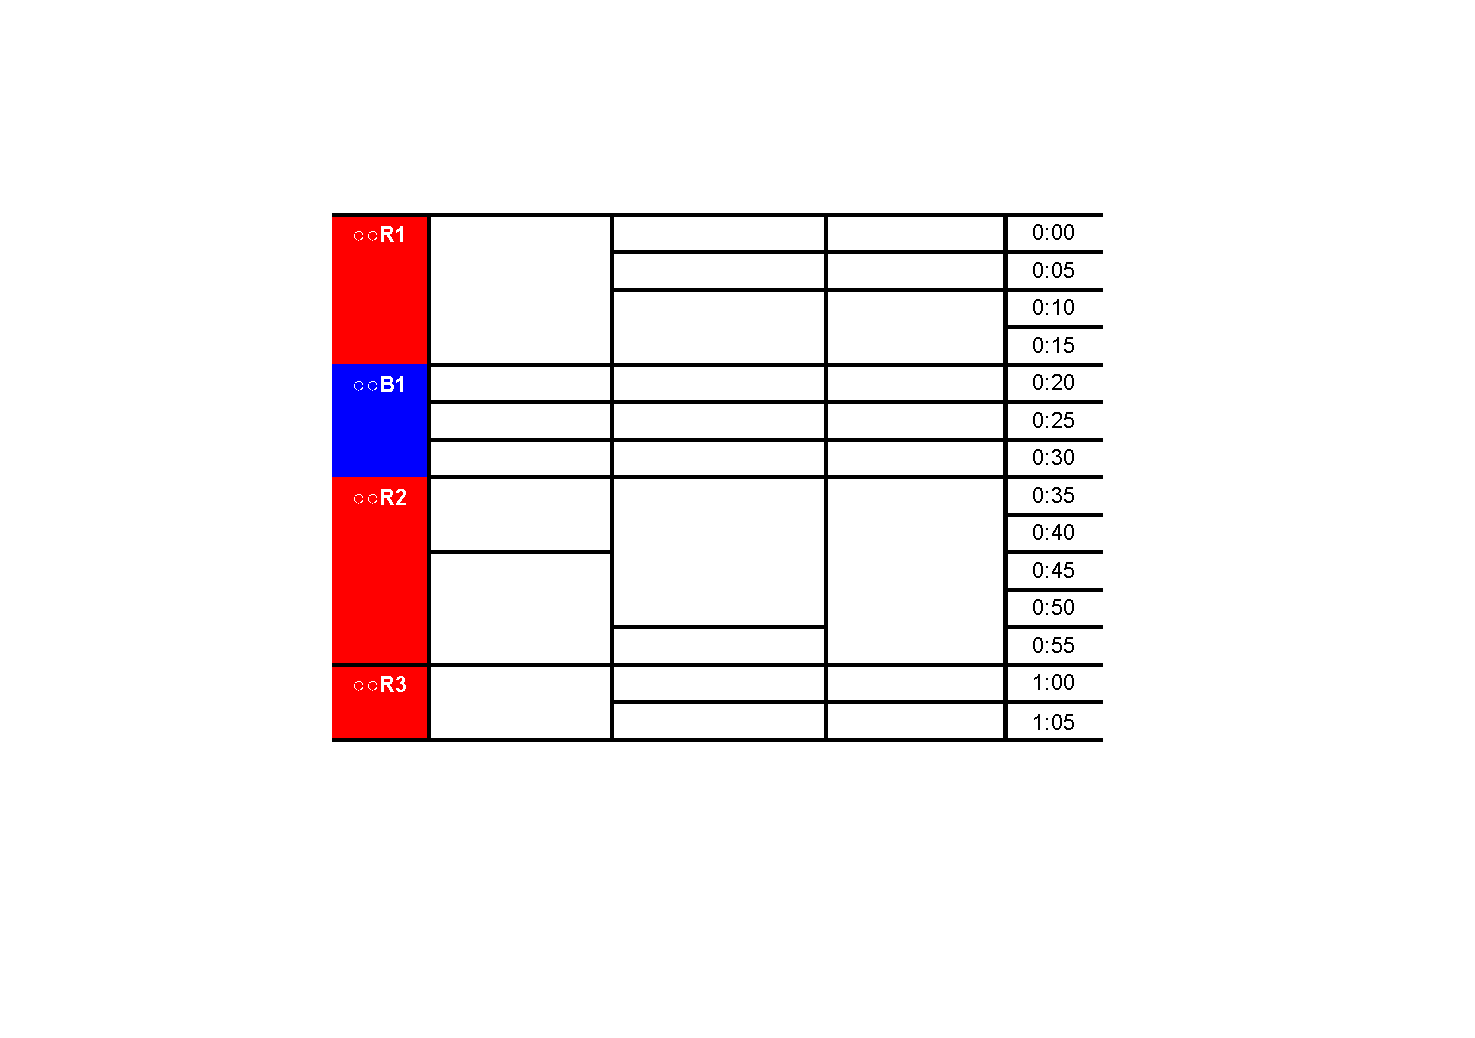
\includegraphics[width=\hsize]{fig/fig1-RB区切り方例.pdf}
\caption{R・B区切り方例}
\label{fig:ｒｂ}
\end{figure}
\subsection{The Two Mouseketeers}
\subsubsection{概要}
この物語は，1952年に公開されたアカデミー賞受賞の短編アニメーション．作品内容として，中世フランスを舞台に，ジェリーとニブルスは小さな剣を持った勇敢な「マウスケティア」として，トムが見張る宮廷の豪華な食事を盗もうとする．トムは晩餐を守る猫の役割を果たすが，ジェリーたちは次々と知恵を駆使してトムを出し抜き，騒動を巻き起こす．

この物語に登場する灰色のネズミは表記ゆれによりタフィーとニブルスという二つの名前がある．本稿では，灰色のネズミはタフィーとする．
\figref{fig:The_Two_Mouseketeers}
\begin{figure*}[tb]
\centering
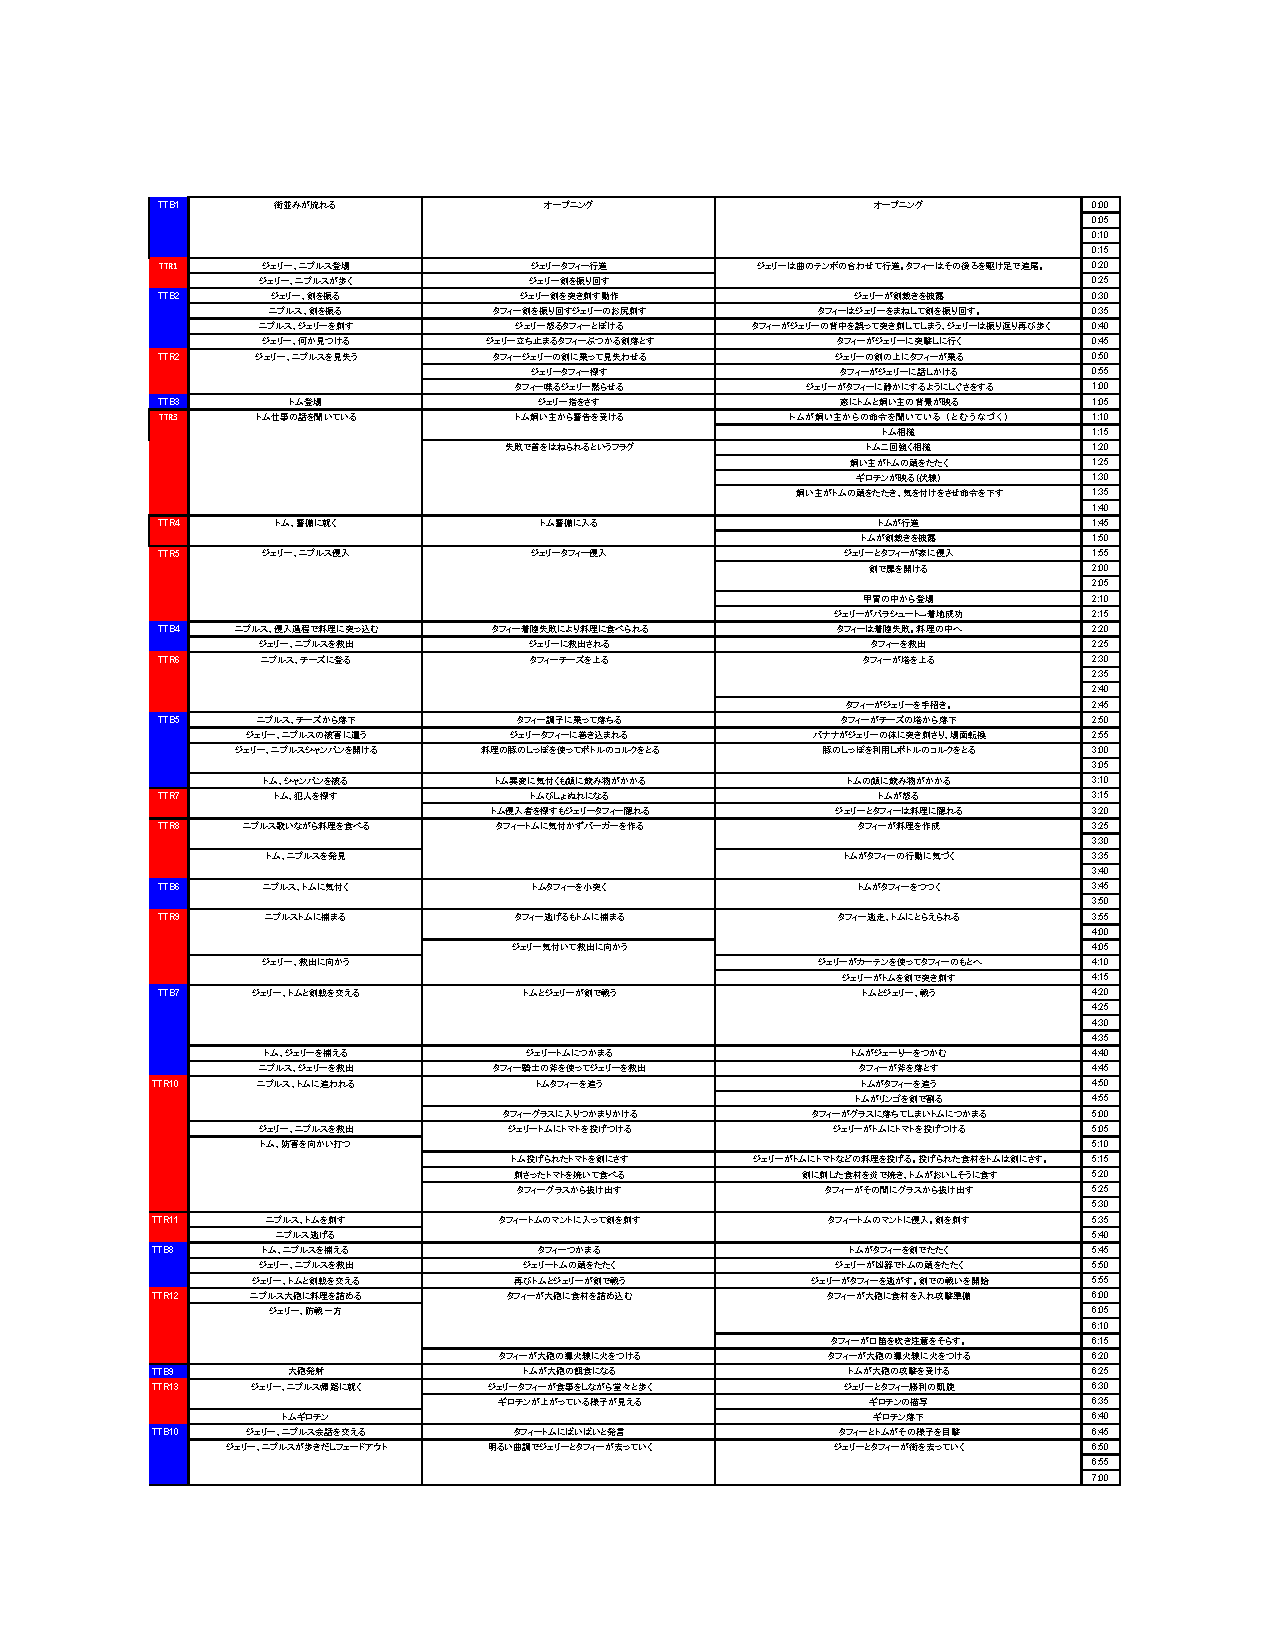
\includegraphics[width=\hsize]{fig/fig2-The_Two_Mouseketeers.pdf}
\caption{The Two Mouseketeers分析結果}
\label{fig:two}
\end{figure*}
\subsubsection{結果・考察}
TTM2では，ジェリーとタフィーが静かにしないといけない状況ということを意識した場合細分化を行っているのではないか．TTR3は，トムの飼い主からの指示の中身を重要視する場合細分化を行う．TTR5では，ジェリーとタフィーが城に侵入するという場面は共通するが，細分化する場合は各登場人物が行っている行動を場面分けしただけだと考える．TTR7は，コルクを当ててきた犯人を捜しにきたトムに対して，トムとタフィーが隠れるという場面であるが，隠れた後に場面転換して次の話になっている．そのため，隠れた後は何も起こっていない．その隠れるという動作に意識したかしていないかで細分化が変ってくる．TTR8は，タフィー視点とタフィーからトム視点に変わっている2パターン存在し，視点が変わっている場面分けの方が細分化される．TTR10は，細分化している方はトムとジェリーの戦いの内容まで意識していて，そうでないほうは戦いの流れを記載している．つまり二匹の戦い自体を広い視点か狭い視点かによって細分化が決まる．

TTB5は，トムとジェリーとタフィーがその物語の中で初めて関わる重要な場面であるため共通して同じ場面分けになったのではないかと考える．TTB9は，タフィーが仕掛けた大砲を発射することによってトムと二匹のネズミとの戦いに決着がつくので物語の中でも印象深い場面となり同じになるのではないかと考える．

\subsection{The Cat Concerto}
\subsubsection{概要}
この物語は，1947年に公開された「トムとジェリー」の短編アニメーションであり，アカデミー賞短編アニメ賞を受賞した作品である．内容として，トムが優雅なコンサートホールでピアニストとして舞台に立つ場面から始まる．彼は観客の前で「ハンガリー狂詩曲第2番」を演奏する．しかし，ピアノの内部にジェリーが住み着いており，演奏中に邪魔を始める．
\figref{fig:The_Cat_Concerto}
\begin{figure*}[tb]
\centering
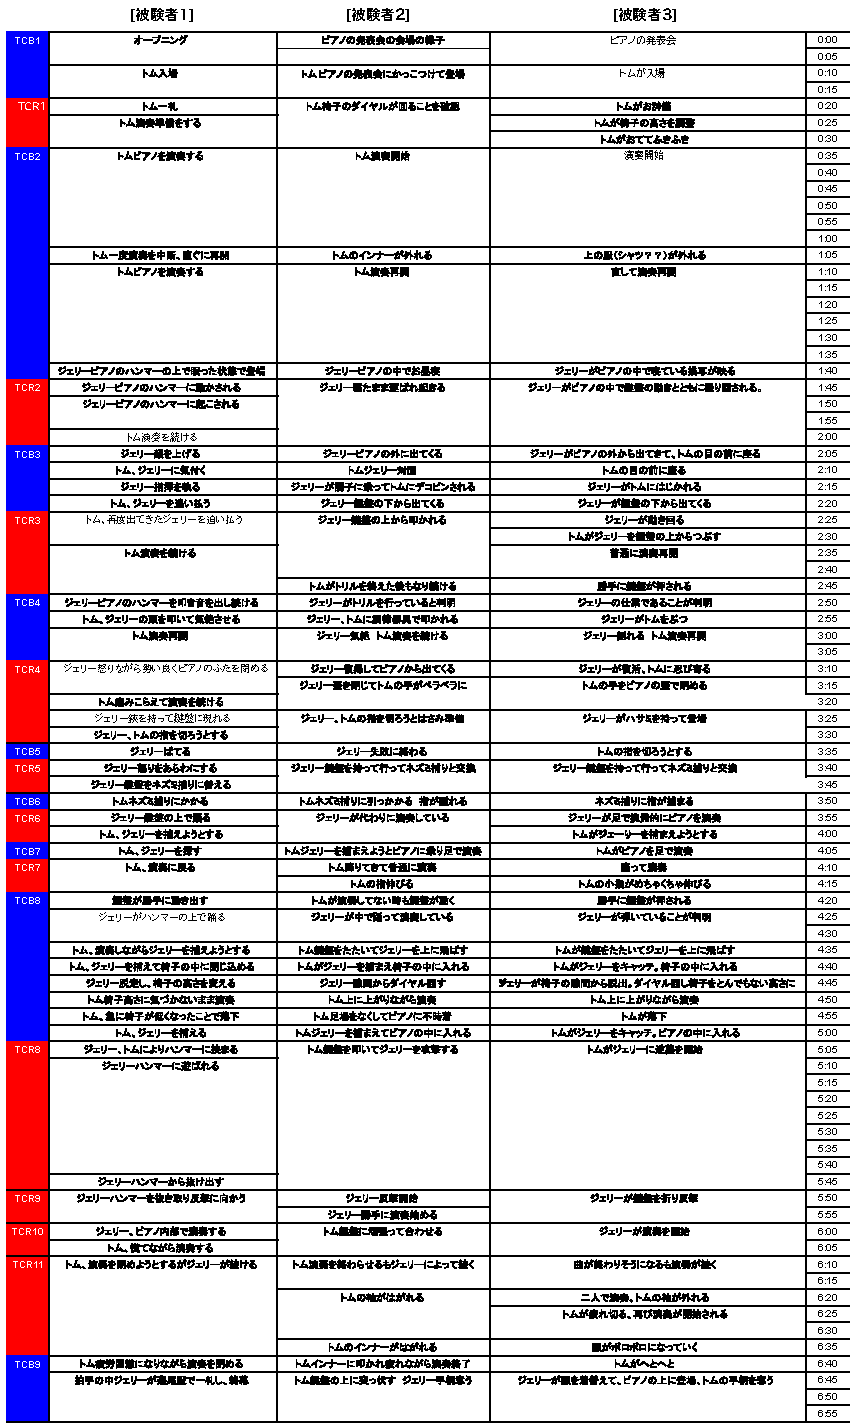
\includegraphics[width=\hsize]{fig/fig3-The_Cat_Concerto.pdf}
\caption{The Cat Concerto分析結果}
\label{fig:concerto}
\end{figure*}
\subsubsection{結果・考察}
TCR２は，場面分けを比較するとトムの行動の記載があるものとそうでないものに分けられる．トムの演奏を追加している場面はトム自身ジェリーに気づいていない状態だと推測される．そのためトムの行動を追加している理由としては第三者視点で物語を観ているのではないかと考える．TCR4は，ピアノのふたをジェリーが閉めた後トムが演奏を続けたということを物語の中で重要視したかどうかで場面分けが変化する．TCR5は，前の場面でトムに仕掛けたことが失敗に終わった後のジェリーが怒るという結果を意識するかどうかで変わる．TCR7は，トムの行動を演奏とひとくくりと解釈しているのか，演奏の中のパフォーマンスとして解釈しているのかで細分化が決まってくる．TCR8は，トムがジェリーに向けて敵意を向けていると解釈した場合攻撃や逆襲などで一つの場面分けになっているが，細分化している場合は，トムがジェリーに対して行ったハンマーにされたことを記載している．TCR10は，細分化されたいないほうは，トムの行動のみとジェリーの行動のみであり，細分化されている方は，ジェリーからトムへと視点が移動している．TCR11は，トムの演奏に対しての「疲労感」を意識するかどうかで，細分化するするかしないかが変化するのではないかと考える．トムの「疲労感」が表面化を表す袖が剥がれたり服がボロボロになったりする場面が追加されるのではないかと考える．

TCR11で述べた服の記載があるものがTCB2でトムの服に対しての記載がある．TCB4で，ジェリーがハンマーをたたいてピアノを鳴らしていることが判明する場面で共通して印象深く感じたのではないかと推測する．TCB6は，前の場面での結果のところであるため被験者が一致して意識して観た場面だと考える．TCB8は，長い間どの場面分けも同じ分け方になり，場面の名称は多少異なるが主語と行動がどの場面も同じになっている．これは，TCB8の場面の流れの中でトムとジェリーで単独で行動する場面が多く，その行動がそれぞれ相手に影響を及ぼしているから同じようになったのではないかと考える．
\subsection{The Missing Mouse}
\subsubsection{概要}
この物語は，1953年に公開された「トムとジェリー」の短編アニメーションである．内容としてトムがジェリーを追いかける中で，ジェリーが白い塗料を浴びて真っ白なネズミに変身する話．ラジオで「危険な放射性ネズミが逃げた」というニュースを聞いたトムは，ジェリーをそのネズミだと勘違いし，大混乱に陥る．
\figref{fig:The_Missing_Mouse}
\begin{figure*}[tb]
\centering
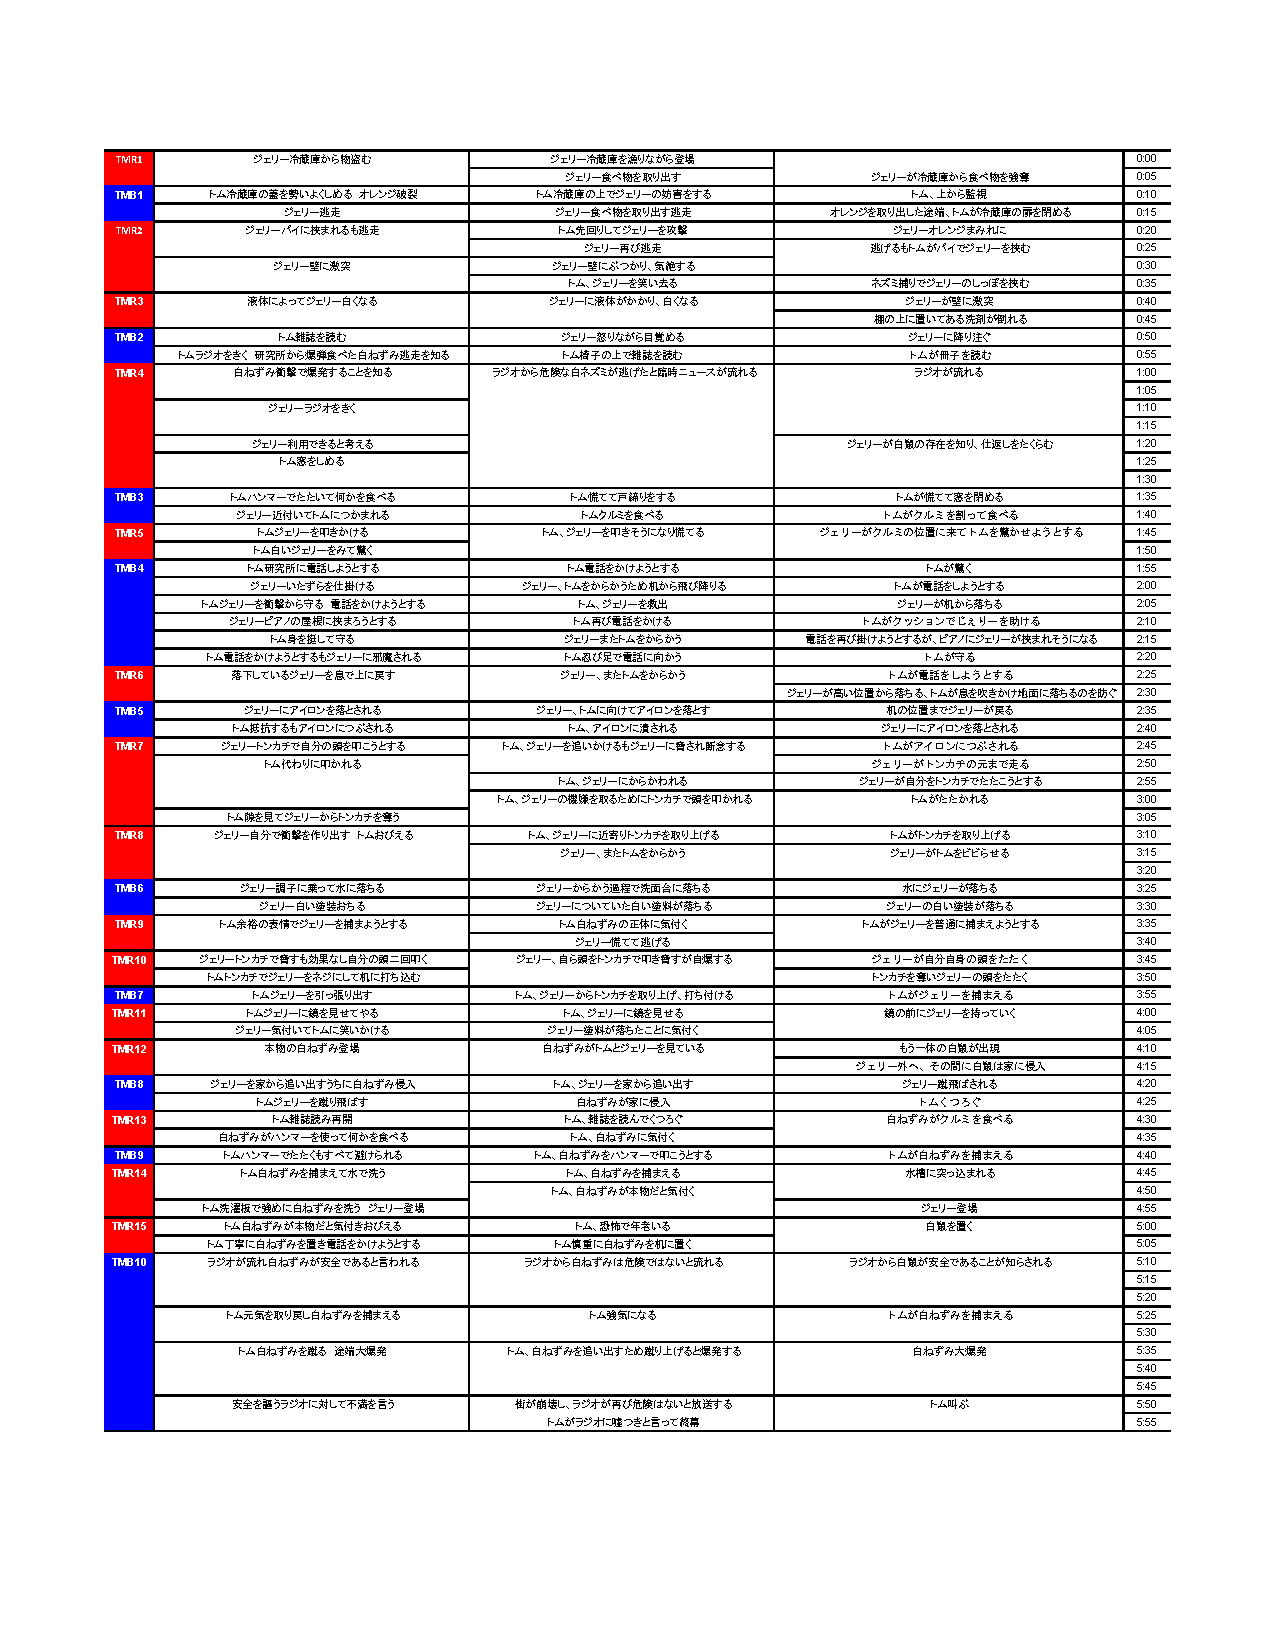
\includegraphics[width=\hsize]{fig/fig4-The_Missing_Mouse.pdf}
\caption{The Missing Mouse分析結果}
\label{fig:missing}
\end{figure*}
\subsubsection{結果・考察}
TMR2で，細分化していないほうはジェリーのみの視点であり，細分化している方は，トムからジェリーへ移動したり逆にジェリーからトムへと視点が移動していたりする．TMR3は，ジェリーが白くなる部分は一緒だが，なぜ白くなったのかの経緯を意識すると細分化が行われる．TMR4は，ジェリーが白いネズミの放送を聞いてその後にトムに対しての行動の理由となるものを意識する場合細分化が行われる．TMR9は，トムがジェリーを捕まえようとした後のジェリーの行動を意識するかどうかで細分化されるか決まる．TMR11は，「ジェリーが鏡を見る」＝「塗料が落ちることに気づく」とするかで塗料が落ちることに気づく場面を設定するか変わっていく．TMR15は，白ネズミが本物と気づいた後の老いていくトムの反応を重要視するかで細分化が変っていく．

TMB4は，ジェリーを白ネズミと勘違いしているトムが爆発させないようにする場面は物語全体でも印象深いため共通するのではないかと考える．TMB6は，ジェリーの白い塗料が落ちトムがジェリーだと気づき，今までの立場が逆転する場面であるため同じになるのではないかと考える．TMB8は，白ネズミがジェリーだったと気づき家には白ネズミがいないと思っているトムに本物の白ネズミが登場する場面であり，白ネズミが話全体で重要であると解釈したためではないかと考える．

\subsection{Mouse Trouble}
\subsubsection{概要}
この物語は，1944年に公開された「トムとジェリー」の短編アニメーションであり，アカデミー賞短編アニメ部門を受賞した作品である．内容としては，トムは，家にいるジェリーを捕まえるために「How to Catch a Mouse」（ネズミ捕獲の秘訣）という本を手に入れ，その指示を忠実に実行しようとする．しかし，ジェリーはトムの企みをことごとく見抜き，巧妙に切り抜けていく．
\subsection{The Missing Mouse}
\subsubsection{概要}
この物語は，1953年に公開された「トムとジェリー」の短編アニメーションである．内容としてトムがジェリーを追いかける中で，ジェリーが白い塗料を浴びて真っ白なネズミに変身する話．ラジオで「危険な放射性ネズミが逃げた」というニュースを聞いたトムは，ジェリーをそのネズミだと勘違いし，大混乱に陥る．
\figref{fig:Mouse_Trouble}
\begin{figure*}[tb]
\centering
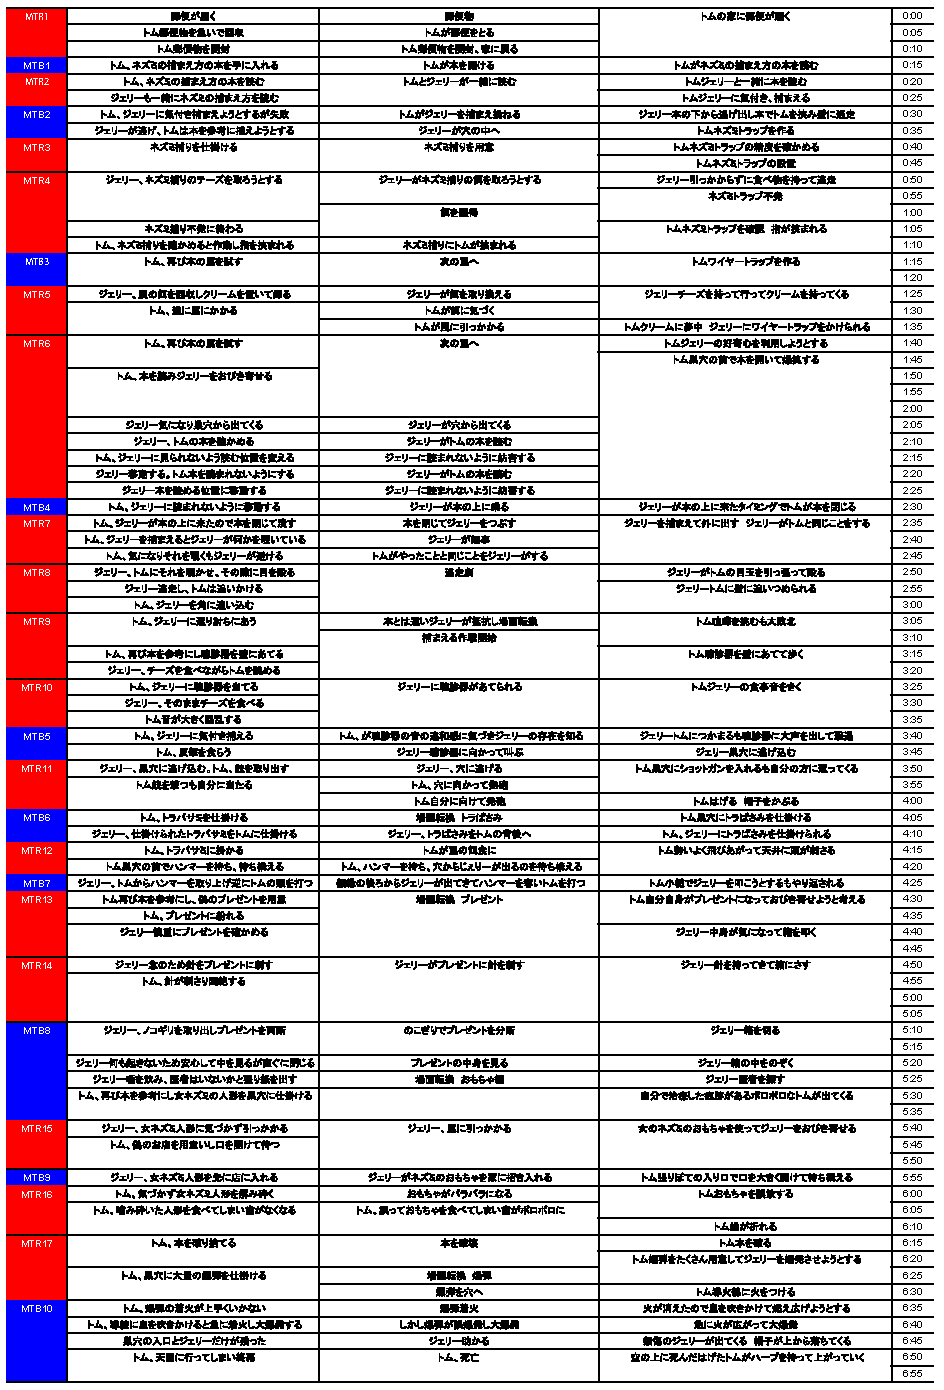
\includegraphics[width=\hsize]{fig/fig5-Mouse_Trouble.pdf}
\caption{Mouse Trouble分析結果}
\label{fig:trouble}
\end{figure*}

\subsubsection{結果・考察}
MTR6は，細分化していないほうは，トムが行った行動のみで，細分化している方は，トムからジェリーへと視点が移動している．さらに細分化している方はジェリーが行った行動に対して細かく場面分けしている．MTR8は，トムとジェリーまとめての行動として場面を解釈しているか，各それぞれのキャラクターの行動としてみているかで細分化されるかが決まっていく．MTR9は，ジェリーを捕まえようとするトムの行動の行動に聴診器を使うという具体性がある場合細分化される．MTR10は，トムがジェリーに聴診器を当てた後のトムの反応を意識する場合細分化がされていく．MTR14は，ジェリーがトムの入っている箱に針を刺す場面であり，トムは映っていないがトムの悲鳴のような音が針を刺すたび鳴る．この音を意識した場合細分化が行われる．MTR15は，トムがどういった経緯でトム自身が仕掛けた罠に引っかかるのかを意識するかどうかで細分化が決まる．

MTB1は，物語の全体の流れとして本を参考にトムがジェリーを捕まえるために罠を仕掛ける．その始まりである本を初めて読む場面であり共通して重要な場面だと解釈したと考える．MTB3も，MTB1と同じように本を参考に罠を仕掛ける場面であるためMTB1と解釈が同じだと考える．MTB8は，トムが入っている箱をノコギリで分断するというショッキングな場面で，どの被験者にも強く印象に残ったためだと考える．

\subsection{対象作品全体の考察}
被験者が観ている視点や行動が単一の場合，場面の細分化はあまり行われないことが多い．一方で，視点や行動が二つ以上存在する場合には，場面が細分化される傾向が顕著であった．特に，視点や行動を示す人物が変更される場合において，場面が細分化される可能性が高まることが確認された．以上の結果は，視点や行動の多様性が場面分けにおける細分化の程度に影響を与えることを示唆している．また，戦闘や演奏といった特定の行動を伴う場面における分析では，その行動が具体的である場合に場面が細分化されやすい傾向が確認された．たとえば，戦闘においては「剣を振る」という動作，演奏においては「鍵盤を叩く」という動作が具体的に描写される際に，場面が細分化される頻度が増加することが観察された．このことから，行動の具体性が場面分けにおける細分化に影響を与える要因の一つであると考えられる． The Cat Concertoのジェリーが怒る場面のような登場人物の感情が現れるところは被験者によって大きく場面分けが変わるポイントであった．

細分化されていない場面分けでは，The Two Mouseketeersのタフィーが放った大砲のようなその物語の状態が劇的に変わるような場面が共通して同じ場面分けになるのではないかと考えた．また，The Missing Mouseのジェリーの塗料が落ちて白ネズミではないことがトムにばれてるような今での登場人物間の関係が変わるような場面は共通して同じ場面になっていった．The Missing Mouseの最後の爆発やMouse Troubleの箱に入っているトムをジェリーがノコギリで分断する場面など強く印象に残るようなところは同じ場面分けになっている．細分化されていない場面に関する分析では，被験者全員が共通して同一の視点や行動を共有している傾向が見られた．このことは，視点や行動の一貫性が場面の細分化を抑制する要因として機能している可能性を示唆している．また，この傾向は，視点や行動が多様化した場合に場面が細分化されやすくなる結果とも整合的であると考えられる．

% ==============
\section{提案}
分析を通して場面分けをする際に以下のことを意識しながら行っていくと直感的にしていたことが根拠をもってできるのではないかと考える．

作品を鑑賞する際，鑑賞者が意識するか否かに関わらず，注目する登場人物は場面ごとに変化する．この注目の変化は，鑑賞者の視点や感情移入の対象が動的であることを示唆しており，作品の分析において重要な要素となる．分析を行う際には，鑑賞者が現在どの登場人物に注目しているのか，または特定の登場人物に注目していない場合には作品全体を俯瞰する第三者的視点で観ているのかを意識することが求められる．この視点の明確化により，場面分けを根拠立てて行うことが可能となる．

「戦い」や「演奏」といった行動の大きなまとまりを捉えるか，あるいはそれを細分化した「剣をふるう」や「サビを弾く」といった個別の行動に焦点を当てるかは，分析の手法や目的に応じて変化する． 大きなまとまりとして行動を捉える場合，その行動全体の意図や結果に着目することが可能となる．一方で，細分化された行動を取り上げることで，具体的な動作や瞬間的な変化を明確にし，より詳細な洞察が得られる．これらのどちらの視点を選択するかは，分析の目的や求められる．

作品において，登場人物たちが行動に移す背景にはさまざまな要因が存在する．その中でも，感情は行動を引き起こす重要な要因の一つであると考えられる．登場人物が抱いた感情がその行動の直接的な動機となっているのか，あるいは他の要因によるものなのかを見極めるこが大切である．感情に基づく行動は，登場人物の内面的な変化や心理的な背景を理解する上で鍵となり得る．一方で，感情に基づかない行動は，別の要因が関与している可能性を示唆する．したがって，分析者は各行動の背後にある要因を精査し，感情との関連性を考える必要がある．

物語において，展開される行動は物語の進行を構築する重要な要素である．その中でも，特に劇的に場面が変化するような行動は，物語の構成において重要な役割を果たしている．そのような行動は，場面分けをする際，意識を向むけることが大切である．

物語において，登場人物間の関係が変化する場面は，物語の流れそのものに変化をもたらす重要な転換点である．このような関係性の変化，物語全体の展開において重要度が高いと考えられる．

場面分けを行う際には，登場人物間の関係がどのように変化し，それが物語の進行や構造にどのような影響を与えているかを意識することが重要である．

作品を鑑賞する際，鑑賞者は喜びや感動といった多様な感情を抱く．その中でも，感情が大きく揺さぶられる場面は，鑑賞者に深い印象を与え，作品の記憶や評価に大きな影響を及ぼす．これらの場面は，物語のクライマックスや転換点であることが多く，鑑賞者の心に強く刻まれる．場面分けを行う際には，このような感情的揺さぶりが生じる場面を特に重視することが求められる．感情の高揚や変化が顕著である場面は，物語の流れやテーマを理解するうえで重要な役割を果たす．

このように，視点，行動の細分化，登場人物の感情や行動や関係性，鑑賞者の感情を意識することで，根拠をもって場面分けができるのではないかと考える．

\section{おわりに}
本研究では，場面分けが根拠的に行う方法について分析，考察を行ってきた．

予備調査として作品分析を行っている論文を収集し，場面分けの現状を調べた．

そのことを踏まえて短編アニメーション作品のトムとジェリーを対象として被験者に場面分けを行ってもらい比較，考察を行った．
その考察を踏まえて根拠をもって場面分けをする方法として視点，行動の細分化，登場人物の感情や行動や関係性，鑑賞者の感情を意識することが大切なのではないかと考えた．
